% Jährlich weltweit erzeugte, kopierte und genutzte Datenmenge (IDC Global DataSphere) in Zettabyte.
% Werte: IDC via Western Digital, zusammengestellt von Statista
% (https://de.statista.com/statistik/daten/studie/267974/umfrage/prognose-zum-weltweit-generierten-datenvolumen/,
% Stand 01.10.2025, abgerufen am 22.11.2026). 2029 ist eine Prognose; die Werte vor 2024 stammen aus älteren IDC-Veröffentlichungen.
% Breite und Höhe richten sich nach \linewidth, damit die Grafik im Skript und auf Folien passt.
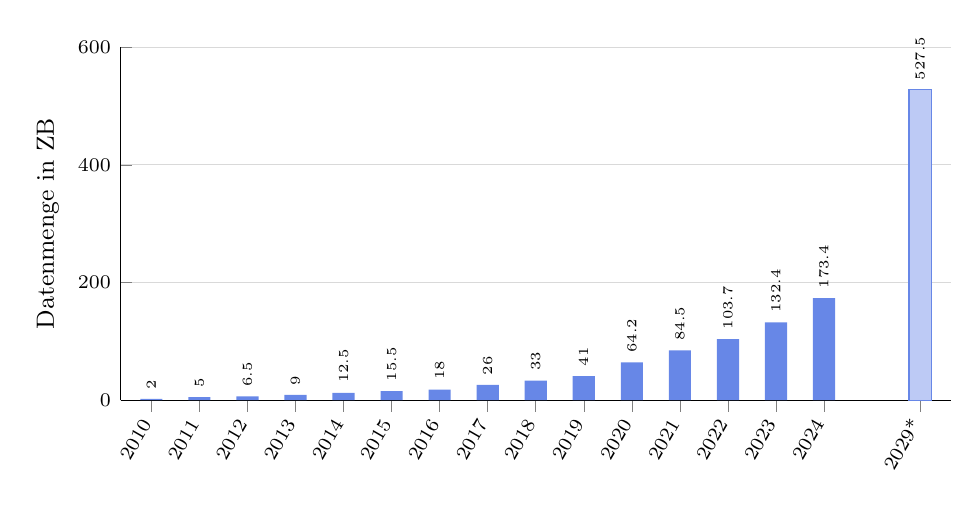
\begin{tikzpicture}
  \begin{axis}[
      width=\linewidth,
      height=.5\linewidth,
      ybar,
      bar width=.8em,
      bar shift=0pt,
      ymin=0, ymax=600,
      ylabel={Datenmenge in ZB},
      % Lücke zwischen 2024 und 2029 als leere Kategorie
      symbolic x coords={2010,2011,2012,2013,2014,2015,2016,2017,2018,2019,2020,2021,2022,2023,2024,gap,2029},
      xtick={2010,2011,2012,2013,2014,2015,2016,2017,2018,2019,2020,2021,2022,2023,2024,2029},
      xticklabels={2010,2011,2012,2013,2014,2015,2016,2017,2018,2019,2020,2021,2022,2023,2024,2029*},
      x tick label style={rotate=60, anchor=east, font=\scriptsize},
      y tick label style={font=\scriptsize},
      ylabel style={font=\small},
      nodes near coords,
      nodes near coords style={font=\tiny, rotate=90, anchor=west},
      point meta=explicit symbolic,
      ymajorgrids, grid style={gray!30},
      axis x line*=bottom, axis y line*=left,
      enlarge x limits=.04,
    ]
    % gemessene bzw. geschätzte Werte bis 2024
    \addplot[fill=RoyalBlue!80, draw=none] coordinates {
        (2010,2) [2] (2011,5) [5] (2012,6.5) [6.5] (2013,9) [9] (2014,12.5) [12.5]
        (2015,15.5) [15.5] (2016,18) [18] (2017,26) [26] (2018,33) [33] (2019,41) [41]
        (2020,64.2) [64.2] (2021,84.5) [84.5] (2022,103.66) [103.7] (2023,132.4) [132.4] (2024,173.4) [173.4]
      };
    % Prognose 2029 (heller dargestellt)
    \addplot[fill=RoyalBlue!35, draw=RoyalBlue!80] coordinates {(2029,527.5) [527.5]};
  \end{axis}
\end{tikzpicture}
